\title{Implicit Matrix Factorization for Recommender systems v0.1}
\date{\today}

\documentclass[12pt]{article}
\usepackage{amsfonts,amsmath,listings, hyperref}
\usepackage{graphicx}
\graphicspath{ {./images/} }
\newcommand{\norm}[1]{\left\lVert#1\right\rVert}
 
\begin{document}
\maketitle

\begin{abstract}
This draft contains theoretical background summary and implementation notes for implicit feedback recommender Proof of Concept based on \cite{CFIFD}. 
Heavily influenced by \href{https://medium.com/recombee-blog/machine-learning-for-recommender-systems-part-1-algorithms-evaluation-and-cold-start-6f696683d0ed}{''Machine Learning for Recommender Systems''} and  \href{https://www.kaggle.com/gspmoreira/recommender-systems-in-python-101/code}{"Recommender Systems in Python 101"}
\end{abstract}

\section{Overview}
Majority of the recommender systems belong to two categories: content-based recommendation and collaborative filtering recommendation. In \cite{CCR} it is mentioned that content based recommendation tries to recommend articles similar to those articles the user has liked, whereas collaborative recommendation tries to find some users who share similar tastes with the given user and recommends articles they like to that user. Content-based recommendation and collaborative recommendation both have their own advantages and drawbacks. But collaborative recommendation is more popular than content-based recommendation, mainly because in many domains it is hard to extract useful features from articles, which is
generally a step required for content-based recommendation.
\subsection{Content Based}
The classical content based approach is to engineer features from the metainformation available for the items in catalog. Once the feature set is ready, it is possible to treat the recommendation problem as a classification problem. This allows one to use more traditional machine learning techniques that output a probability for a certain user to like a specific item based on a training set of their purchase history. Then, items are re-ranked using predicted scores and top $n$ are recommended.

\subsection{Associative rules mining}
Market Basket Analysis is one of the key techniques used in commerce to uncover associations between items. 
The idea is to look for combinations of items that occur together frequently in transactions. This allows retailers to identify relationships between the items that people buy.

Association Rules are widely used to analyze retail basket or transaction data, and are intended to identify strong rules discovered in transaction data using measures of interestingness, based on the concept of strong rules.

The framework of association rules was introduced into the data mining community at large by Agrawal et al. \cite{AZM}. A large variety of association rule mining algorithms have been published in the literature, including Apriori.   Adaptive-support algorithm to mine association rules for recommender systems is an evolution from the Apriori and CBA-RG algorithms and is presented in \cite{LAR}.

\subsection{Collaborative Filtering}
Collaborative filtering approach is based on the exploiting the relationship between users and items, with no meta-information or hand-crafted features about the users or the items required All that is required is a "rating" (for explicit matrix factorization) or "preference" (for implicit matrix factorization) of some kind for each user/item interaction that occurred where available. There are two kinds of data available for this type of interaction: explicit and implicit.

\begin{itemize}
	\item Explicit: An epxlicti score, such as a rating or a like
	\item Implicit: Not as obvious in terms of preference, such as a click, view, or purchase
\end{itemize}

The most widely studied toy example is movie ratings, where explicit ratings are given on a numeric scale. We can easily see whether a user enjoyed a movie based on the rating provided. The problem, however, is that in case of e-retail people frequently leave a lot of comments and the interactions with the item and web-sit itself must be considered as a source of implicit type of feedback.

Since more data usually means a better model, implicit feedback is where our efforts should be focused. While there are a variety of ways to tackle collaborative filtering with implicit feedback, I will focus on the method included in Spark’s library used for collaborative filtering, alternating least squares (ALS).

\section{Implicit and Explicit latent factor models}\label{overview}
Contents of the section is a brief summary of section of the classical paper  \cite{CFIFD}.
\subsection{Explicit feedback. Model based Collaborative filtering}
Let us assume that we have a user-by-item matrix where nonzero elements of the matrix are the {\it{explicit ratings}} that a user has given an item. We assume that the rank of the ratings matrix allows (strict details are required here, Eckart–Young–Mirsky ???) us to approximate: 
\begin{itemize}
\item each user by k attributes or features
\item each product by k attributes or features. 
\end{itemize}
\begin{figure}[h]
\caption{taken from cs246 Stanford}
\includegraphics[width=0.9\textwidth]{cs246_model_m_factor}
\end{figure}
the scalar product of the dense factor of the users by the corresponding dense factor of the product  this will be a good approximation for the rating the user would give that product.

The problem of the approximation can be posed as a minimization problem. Let us define per each user $u \in \mathcal{U}$ a latent factor vector $\vec{x}_u \in \mathbb{R}^k$ and for each item  $i \in \mathcal{I}$ a latent factor $\vec{y}_i \in \mathbb{R}^k$. Then user predicted rating ($\hat{\cdot}$ denotes prediction) would be 
\begin{equation}
\hat{r}_{ui} = (\vec{x}_u, \vec{y}_i)
\end{equation}
In this setting the functional of choice to minimize would be :
\begin{equation}
\mathcal{L} = \sum_{u \in \mathcal{U}, i \in \mathcal{I}} 
\left\{r_{u,i}-(\vec{x}_u, \vec{y}_i)\right\} ^2
+ 
\lambda_x \sum_{\mathcal{U}}\norm{\vec{x}_u}^2
+ 
\lambda_y \sum_{\mathcal{U}}\norm{\vec{i}_i}^2
\end{equation}

\subsection{Explicit model. Alternative Least Squares}\label{eals}
For ALS procedure, one would proceed in a manner similar to stochastic gradient descent but a bit smarter. We iteratively would freeze one of the latent vectors and solve with respect to the others. For example one can start with item vectors. If items vectors are considered to be frozen, it is possible to  take the derivative of the loss function with respect to user latent vectors. Solving the equation given by the equating of the derivative to zero and freezing the variable makes it possible to proceed with {\it{alternative step}} and solve for the items. The process is repeated until convergence achieved \ref{On the Convergence of Alternating Least Squares Optimisation in Tensor Format Representations}
\begin{equation}
\frac{\partial \mathcal{L}}{\partial \vec{x}_u}  = -2 \sum_{i \in \mathcal{I}} \left(r_{u,i}-(\vec{x}_u, \vec{y}_i)\right) \vec{y}_i^T+
2\lambda_x \vec{x}_u^{T}
\end{equation}
Setting derivative to zero leads to 
\begin{equation}
\vec{x}_u^T  = \vec{r}_u\mathbb{Y}\left(\mathbb{Y}^T\mathbb{Y}+\lambda_x\mathbb{I}\right)^{-1}
\end{equation}
Similar calculations lead to (in case of frozen user factors) to:
\begin{equation}
\vec{y}_i^T  = \vec{r}_i\mathbb{X}\left(\mathbb{X}^T\mathbb{X}+\lambda_y\mathbb{I}\right)^{-1}
\end{equation}
Having written explicitly equations one can proceed with iteration procedure. But since we are interested in implicit case, let us move forward.

\section{Implicit Alternative Least Squares}\label{ials}
The transactional data that is readily available in Oracle is implicit. The simplest way to treat the implicit feedback signals is to assume that a user  buying a product signals that the user likes a product, the catch here is that with this approach there is no notion of a negative signal. Not having data does not mean that user does not like the product, it might simply indicate that user never encountered the product that otherwise might be of interest. This means we can't just treat the missing data as unknowns, instead we have to treat a user not buying an item as being a signal that the user {\it might} not like that thing.

This presents a couple of challenges in learning a factorized representation. Summary according to \cite{CFIFD}
\begin{itemize}
\item No negative feedback
\item Implicit feedback is inherently noisy
\item The numerical value of explicit feedback indicates {\it preference}, whereas the {\textbf{numerical value of implicit feedback indicates {\it confidence}}}
\end{itemize}

The Collaborative Filtering for Implicit Feedback Datasets provides elegant recipes to treat all the items.

The crucial difference with the explicit case is handling the case where we're not confident about our negative data. Suggested approach learns a factorized matrix representation using different confidence levels on binary preferences: unseen items are treated as negative with a low confidence, where present items are treated as positive with a much higher confidence.

In order to proceed let us first define the following quantities: $u,v$ will be index letters for users and $i, j$ will be indexes for items. The input data that associate user purchases with items will be represented by a matrix $\mathbb{R} = {r_{u,i}}$, $\forall u \in \mathcal{U}, i \in \mathcal{I}$  (the observed sets). In contrary to explicit case we would not treat as unknown unobserved interaction between user and items but explicitly set them to zero. In addition let us introduce the notion of confidence which the given values of $r_{u,i}$ measure. To this end, following \cite{CFIFD} let us introduce the binary value $p_{u,i}$ which indicates the preference of user $u$ to item $i$

\begin{equation}
p_{u,i} = \begin{cases}
    1, & \text{if $r_{u,i}>0$}.\\
    0, & \text{if $r_{u,i}=0$}.
  \end{cases}
\end{equation}
Basically our preference is a binary representation of our feedback data $r_{u,i}$. If the feedback is greater than zero we set it to 1.
Now the idea is to combine the preference $p$ for an item with the confidence $c$ we have for that preference. We start out with missing values as a negative preference with a low confidence value and existing values a positive preference but with a high confidence value. The confidence is set up as strictly monotone increasing function of feedback data. In our case, following the paper, we will have it as linear one
\begin{equation}
c_{u,i} = f(r_{u,i}) = 1 + \lambda r_{u,i}
\end{equation}

Effectively this means that we have a larger confidence the more times a user has bought an item. We also add 1 so we have a minimal confidence even if  $r_{u,i}$ equals zero. 

The goal now is to find the vector for each user $\vec{x}_u$ and item $\vec{y}_i$ in feature dimensions which means we want to minimize the following loss function:

\begin{equation}
\mathcal{L} = \sum_{u \in \mathcal{U}, i \in \mathcal{I}} 
c_{u,i}\left\{r_{u,i}-(\vec{x}_u, \vec{y}_i)\right\} ^2
+ 
\lambda \sum_{\mathcal{U}}\norm{\vec{x}_u}^2
+ 
\lambda \sum_{\mathcal{U}}\norm{\vec{i}_i}^2
\end{equation}
\subsection{ALS for implicit feedback}
Following the paper and freezing sequentially items and user we arrive at
\begin{equation}
\vec{x}_u = \left(
\mathbb{Y}^TC^u\mathbb{Y} + \lambda\mathbb{I}
\right)^{-1}\mathbb{Y}^TC^u p_u
\end{equation} 
and similarly
\begin{equation}
\vec{y}_i = \left(
\mathbb{X}^TC^u\mathbb{X} + \lambda\mathbb{I}
\right)^{-1}\mathbb{X}^TC^u p_i
\end{equation} 
One can note that computing $\mathbb{Y}^TC^u\mathbb{Y}$ is an expensive operation. Thankfully this can be represented as 
\begin{equation}
\mathbb{Y}^TC^u\mathbb{Y} = \mathbb{Y}^T\mathbb{Y}+ \mathbb{Y}^T\left(C^u-\mathbb{I}\right)\mathbb{Y}
\end{equation}
and since $ \mathbb{Y}^T\mathbb{Y}$ is independent of $u$ it can be precomputed that drastically speeds up processing time.

Now the algorithm to follows becomes fully straightforward:
\begin{itemize}
\item Randomly initialize user and item factor matrices. 
\item $\lambda$ manually select regularization parameter. Theoretically we have to do hyper-parameter swipe
\item iterate between two above-stated equations
\end{itemize}
\newpage
\section{Case studies}
\begin{figure}[h]
\caption{Cat specific case. Working code is available in the jupyter notebook}
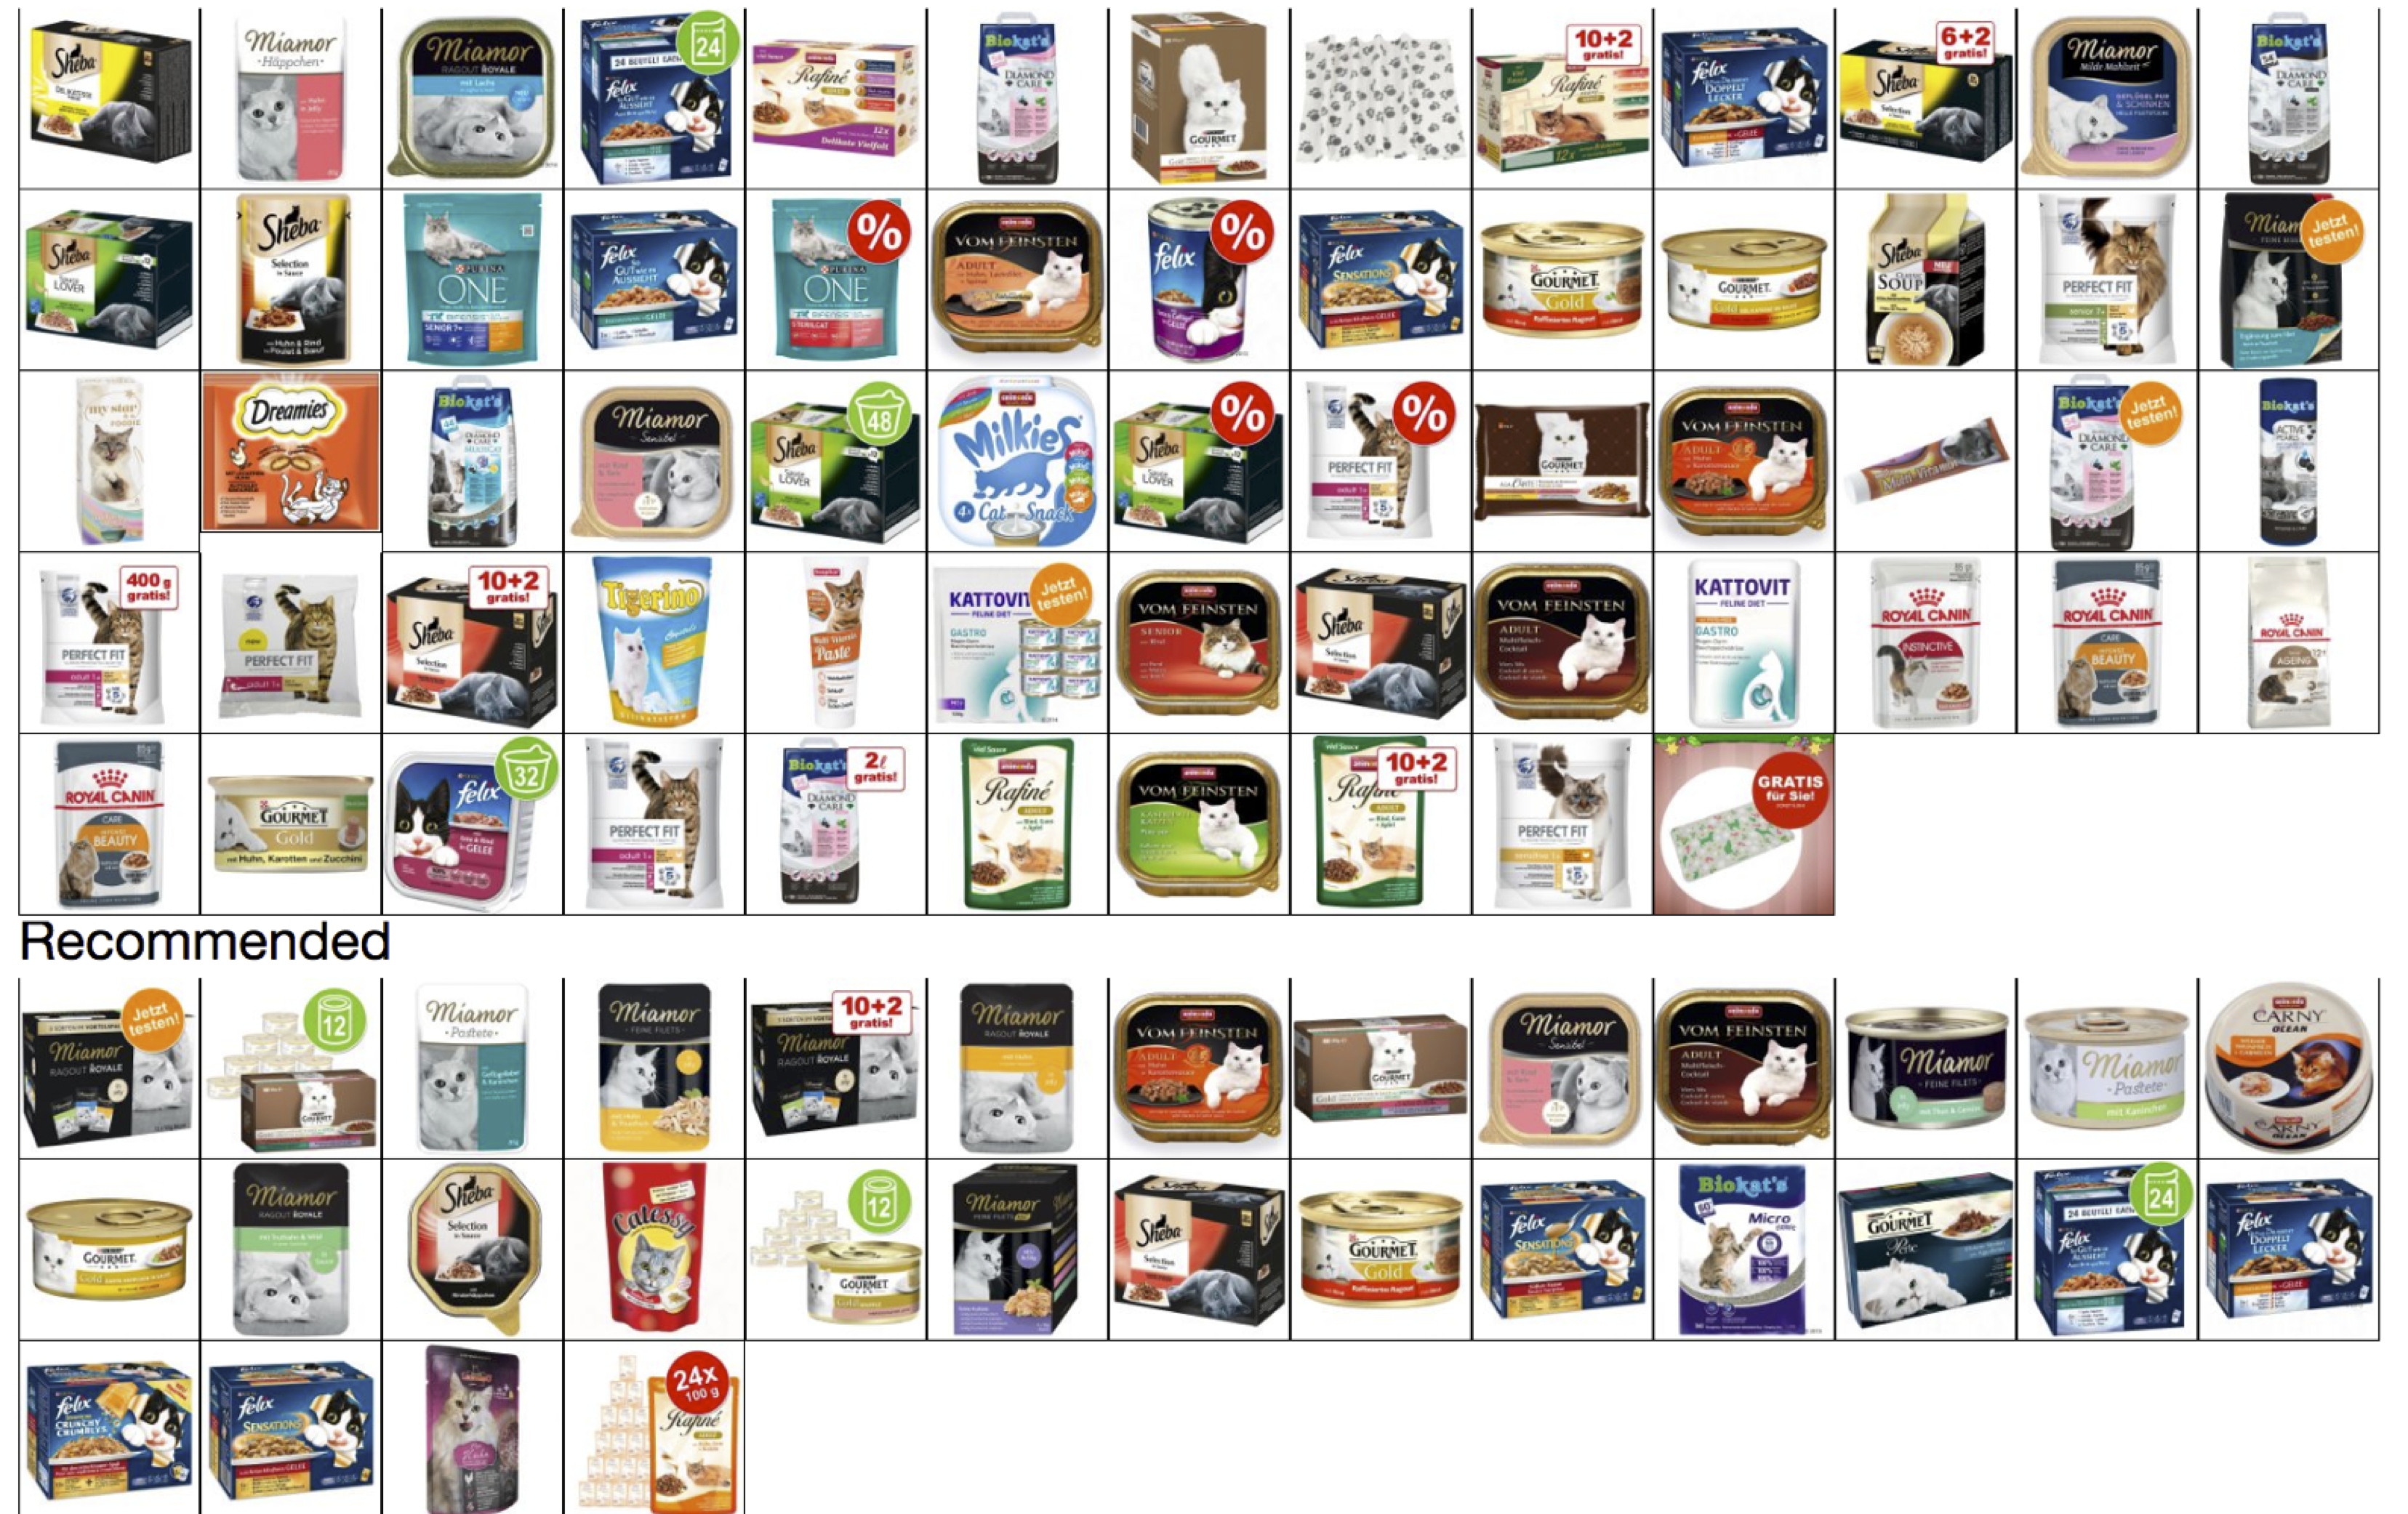
\includegraphics[width=0.9\textwidth]{catonly}
\end{figure}
\newpage
\begin{figure}[h]
\caption{Mixed with dog bias specific case. Working code is available in the jupyter notebook}
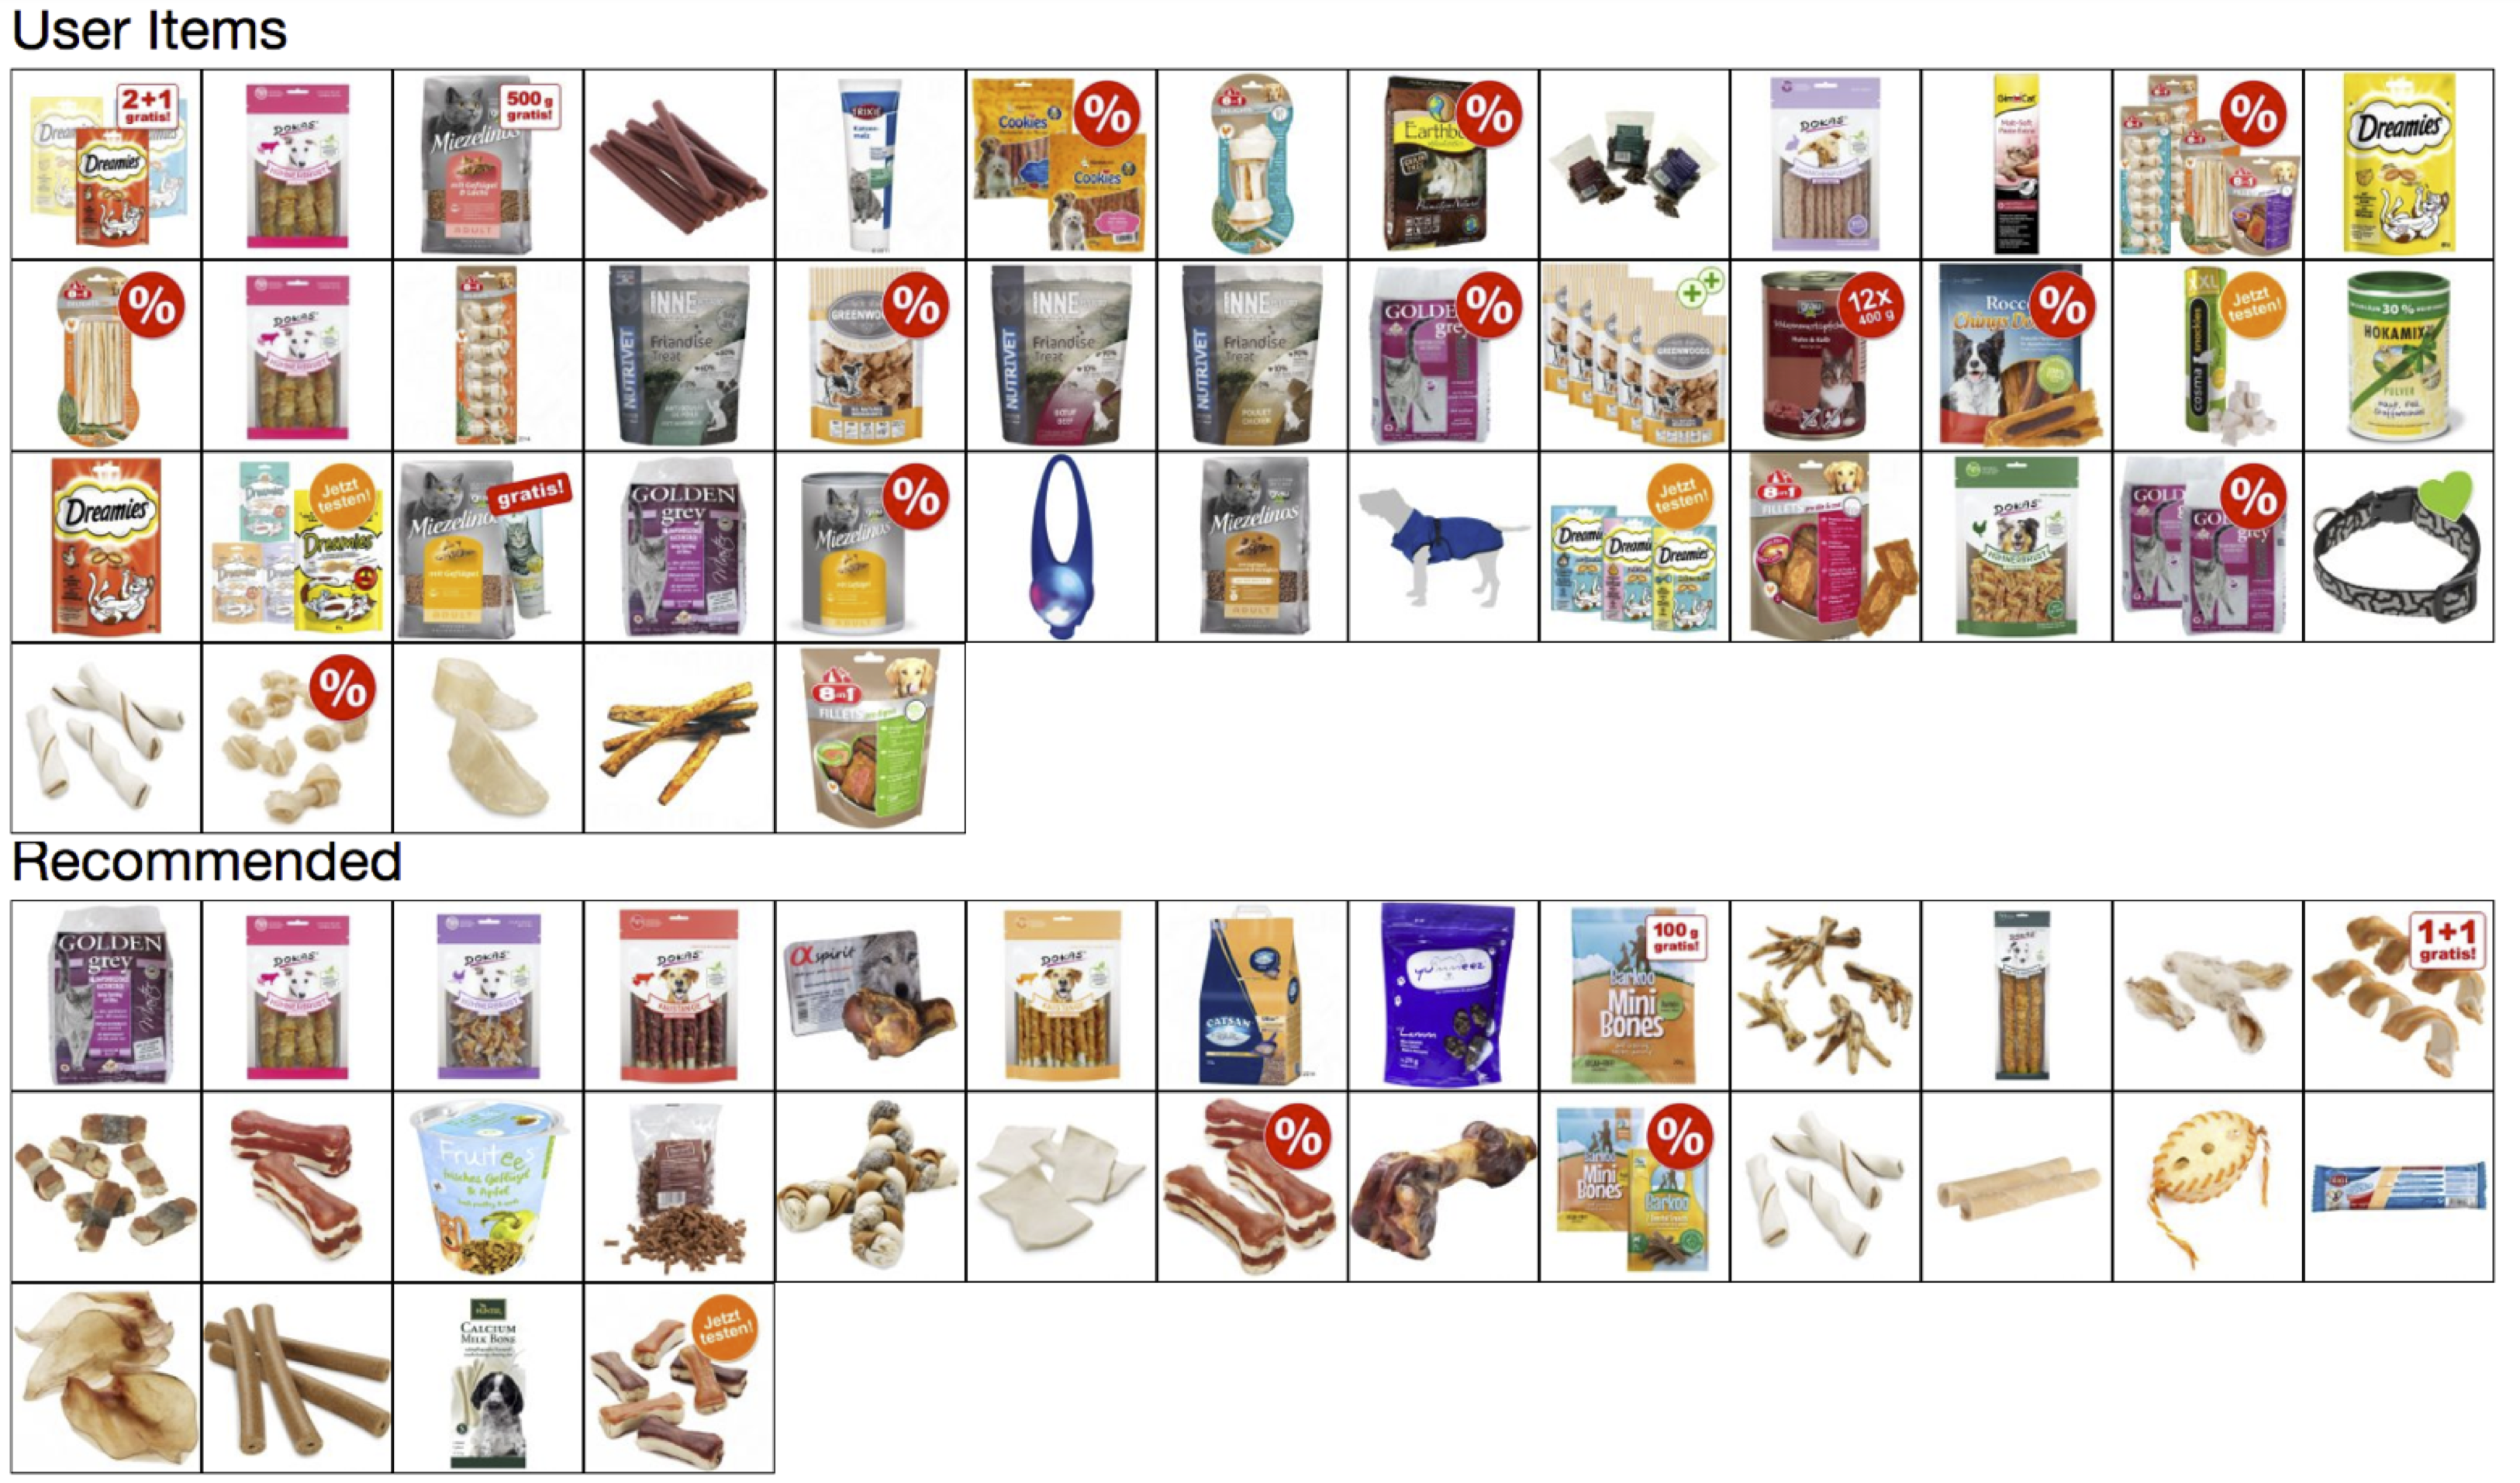
\includegraphics[width=0.9\textwidth]{dogplussomecat}
\end{figure}
\newpage
\begin{figure}[h]
\caption{Dog specific case. Working code is available in the jupyter notebook}
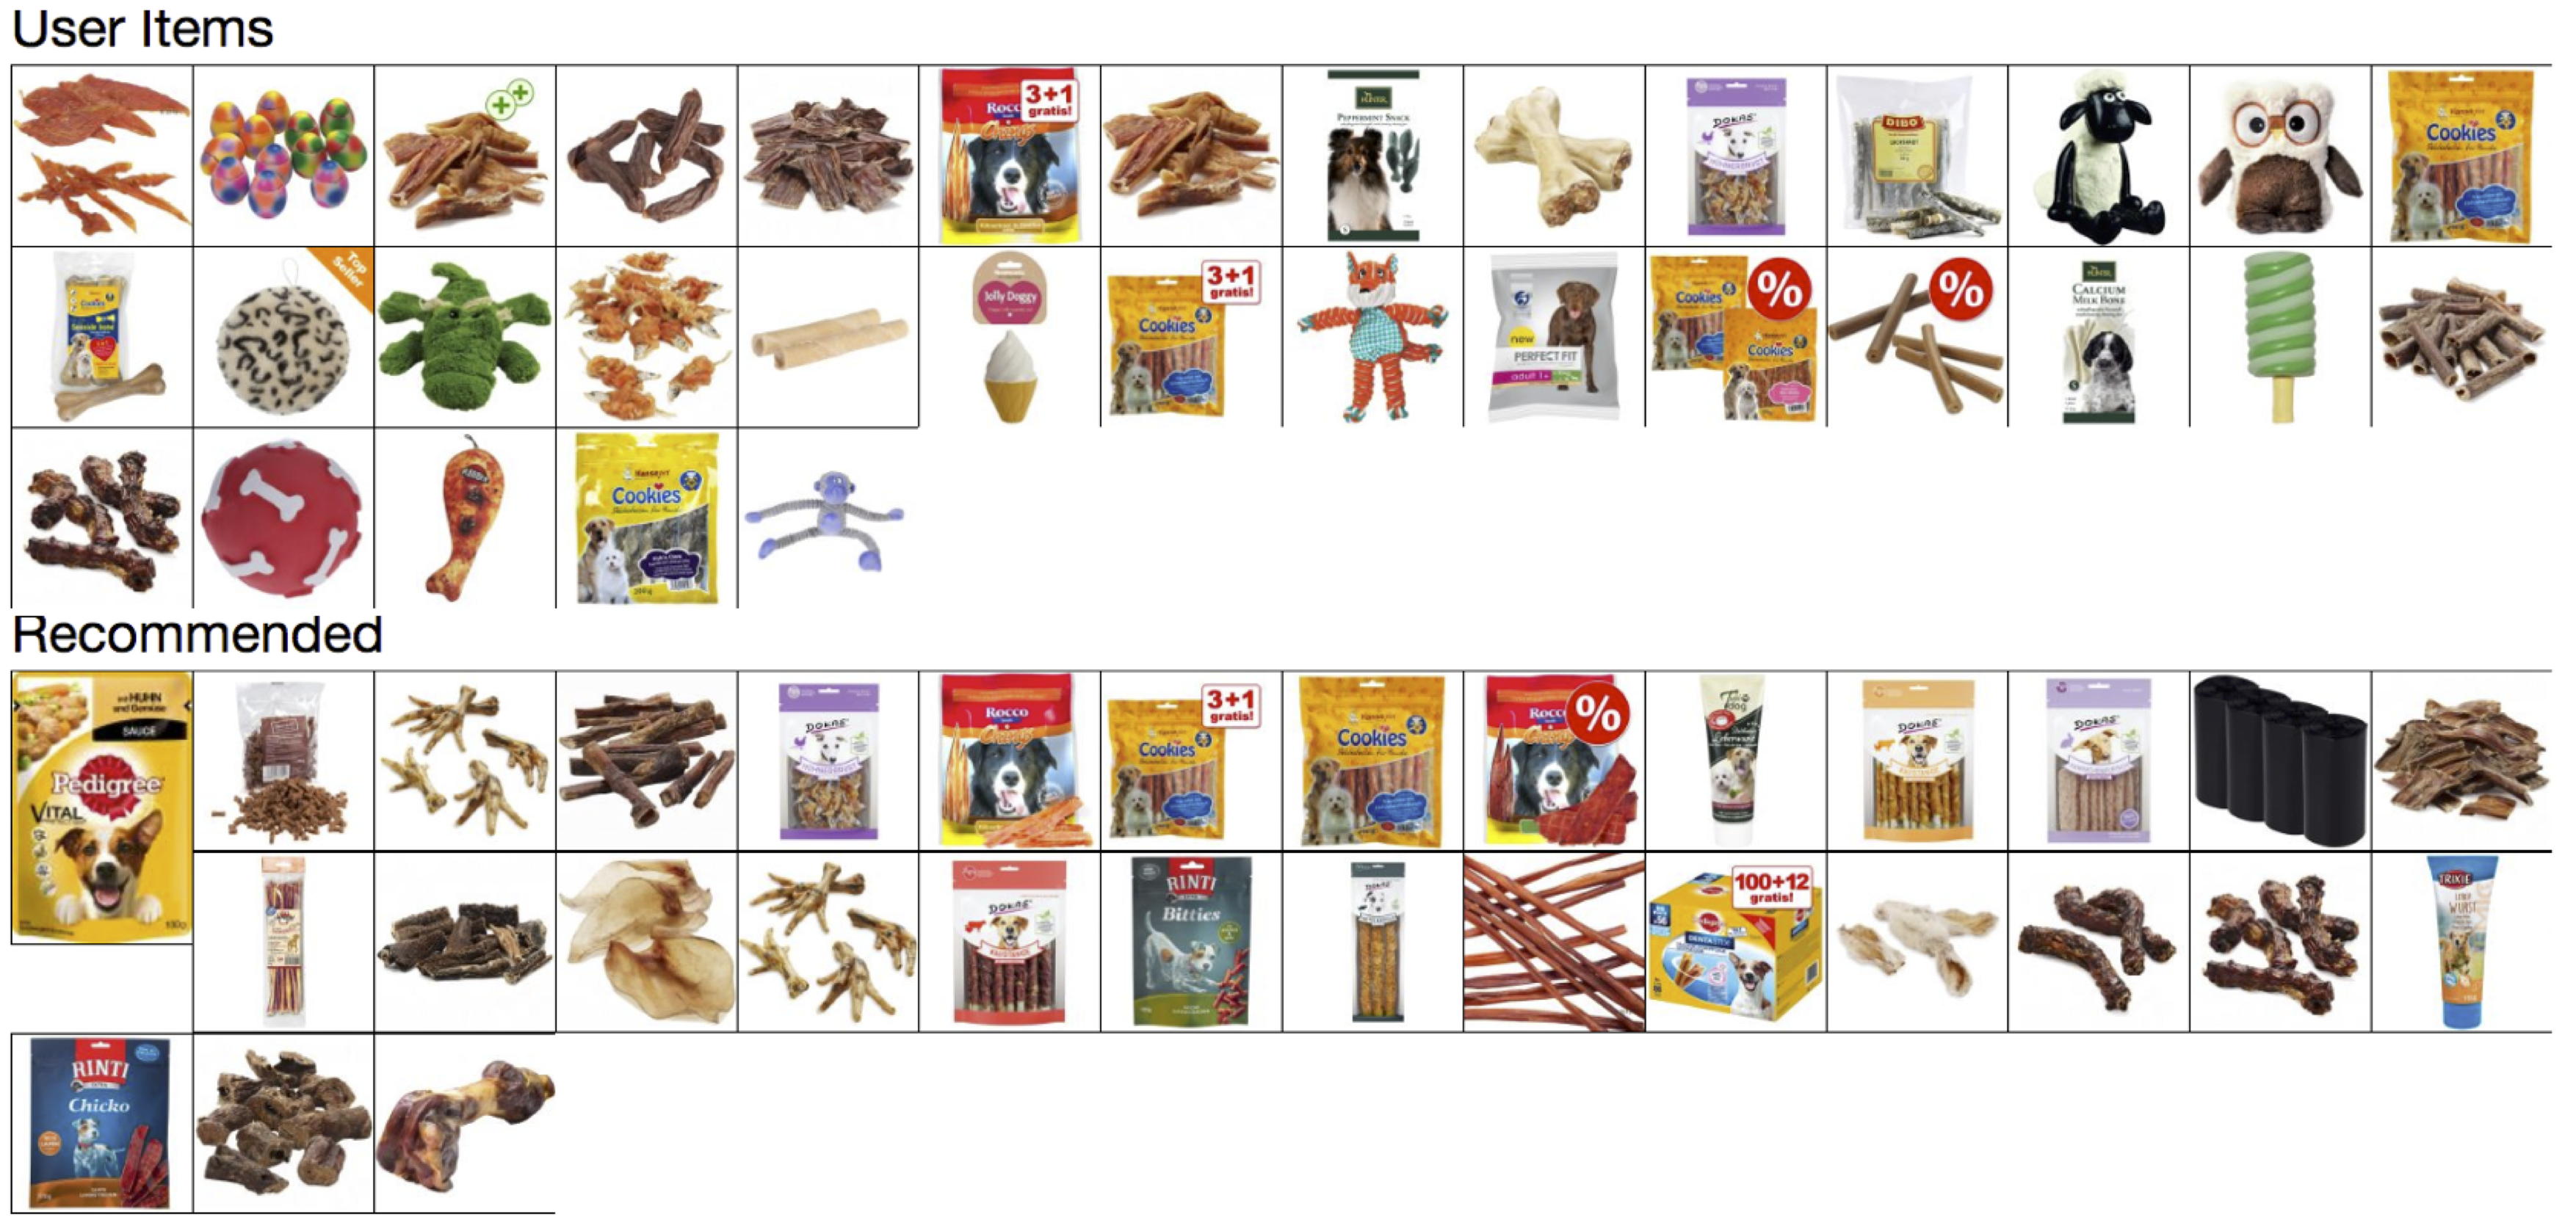
\includegraphics[width=0.9\textwidth]{dogsnacks}
\end{figure}
\newpage
\section{Appendix (not tested): 100 lines implementation with SciPy solver}
While writing this document I have stumbled upon a scipy solver and using it the implementation of the algorithm could actually fit on a couple of pages. It is actually fast and according to scipy documentation designed to work with sparse matrices. In the notebook I am using a Conjugate gradient solver written in Cython.
\begin{lstlisting}[language=Python]
import random
import numpy as np

import scipy.sparse as sparse
from scipy.sparse.linalg import spsolve

class ImplicitAlternativeLeastSquares():

    def __init__(self, embedding=10, alpha=40,
    		 iterations=10, lambda=0.1):
        self.embedding = embedding
        self.alpha = alpha
        self.iterations = iterations
        self.lambda = lambda
        # random initialization
        self.X = sparse.csr_matrix(
            np.random.normal(size=(user_dim, embedding)))
        self.Y = sparse.csr_matrix(
            np.random.normal(size=(item_dim, embedding)))
            self.X_I = sparse.eye(user_dim)
            self.Y_I = sparse.eye(item_dim)

    def _calulate_binary_pref(p, row):
        p = row.copy()
        p[p != 0] = 1.0

    def sparse_ials(self, data):
        user_dim, item_dim = data.shape

        I = sparse.eye(embedding)
        lI = lambda * I
        c = alpha * data  # setting up confidence
        # Alternation
        for i in tqdm(range(iterations)):

            # Precompute transpose products
            yTy = self.Y.T.dot(self.Y)
            xTx = self.X.T.dot(self.X)

            for u in range(user_size):
                u_row = c[u, :].toarray()

                self._calculate_binary_pref(p_u, u_row)

                # Calculate Cu and Cu - I
                CuI = sparse.diags(u_row, [0])
                Cu = CuI + self.Y_I

                # Put it all together and compute the final formula
                yTCuIy = self.Y.T.dot(CuI).dot(self.Y)
                yTCupu = self.Y.T.dot(Cu).dot(p_u.T)
                self.X[u] = spsolve(yTy + yTCuIy + lI, yTCupu)

            for i in range(item_size):
                i_row = c[:, i].T.toarray()

                self._calculate_binary_pref(p_i, i_row)

                # Calculate Ci and Ci - I
                CiI = sparse.diags(i_row, [0])
                Ci = CiI + self.X_I

                # Put it all together and compute the final formula
                xTCiIx = self.X.T.dot(CiI).dot(X)
                xTCipi = self.X.T.dot(Ci).dot(p_i.T)
                self.Y[i] = spsolve(xTx + xTCiIx + lI, xTCipi)

        return self.X, self.Y

\end{lstlisting}


\bibliographystyle{abbrv}
\bibliography{main}
\begin{thebibliography}{9}
\bibitem{CFIFD} 
Yifan Hu, Yifan Hu,  Chris Volinsky. 
\textit{Collaborative Filtering for Implicit Feedback Datasets}. 
AAAI Technical Report WS-98-08. Compilation copyright © 1998, AAAI 

\bibitem{CCR} 
Marko Balabanovic and Yoav Shoham. 
\textit{Content-based, collaborative recommendation.}. 
Communications of the ACM, 40(3):66–72, March 1997


\bibitem{AZM} 
Deepak Agarwal, Liang Zhang, and Rahul Mazumder 
\textit{Modeling item–item similarities for personalized recommendations on Yahoo! front page}. 
Ann. Appl. Stat. Volume 5, Number 3 (2011), 1839-1875.


\bibitem{LAR} 
Weiyang Lin, Sergio A. Alvarez,  Carolina Ruiz
\textit{Collaborative Recommendation via Adaptive Association Rule Mining}. 

 \end{thebibliography}

\end{document}